\chapter{傅立叶分析}
\begin{flushright} \it 跟我读:傅立叶就是爱好大半夜在数字电视上看笨蛋测验召唤兽 \\ 第四卷,但这样做注定会为顺利订购必胜客外卖制造致命障碍。 \end{flushright}
\section{用三角函数拼出奇怪的东西}
一个三角函数(这里指正弦函数或者余弦函数)的图像我们都很熟悉,两个相同频率的三角函数加起来还是相同频率的三角函数。但是把不同频率的三角函数加起来,图像就会变复杂。比如$f(x)=\sin x+2 \sin 2 x+3 \sin 3 x+4 \cos 4 x+5 \cos 5 x$,它的图像如图\ref{fig-trigo-sum}。
\begin{figure}[htb]
\centering
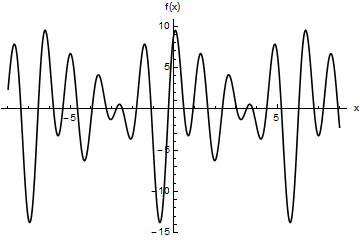
\includegraphics[scale=0.5]{fig/trigo-sum}
\caption{一坨三角函数}
\label{fig-trigo-sum}
\end{figure}

把无穷多个三角函数加起来会变成一个方波:
\begin{equation*}
f(x)=\frac{4}{\pi} \sum_{n=0}^{\infty} \frac{1}{2 n+1} \sin (2 n+1) x=\frac{4}{\pi} \sin x+\frac{4}{3 \pi} \sin 3 x+\frac{4}{5 \pi} \sin 5 x+\dots
\end{equation*}

虽然这个式子又有无穷级数又有$\pi$,但是不要怕,待会就要讲它是怎么算出来的。图\ref{fig-trigo-square-wave}分别是前$3$、$6$、10项的图像。可以证明,如果把无穷多项加起来,图像就会无限接近方波。
\begin{figure}[htb]
\centering
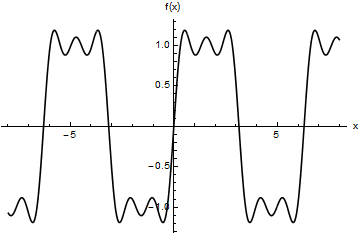
\includegraphics[scale=0.4]{fig/trigo-square-wave}
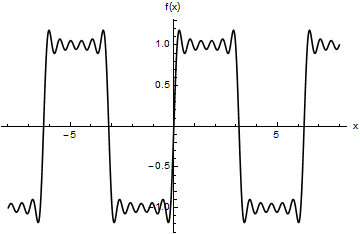
\includegraphics[scale=0.4]{fig/trigo-square-wave-2}
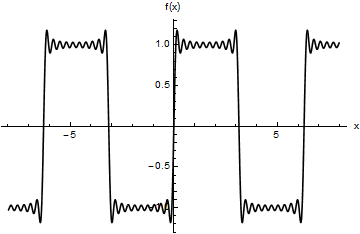
\includegraphics[scale=0.4]{fig/trigo-square-wave-3}
\caption{越来越有方波的感觉了}
\label{fig-trigo-square-wave}
\end{figure}

这个方波的振幅为$1$,最小正周期为$2 \pi$。改变振幅只要乘一个常数就行了。如果要把最小正周期改成$T$,可以把$x$改成$\frac{2 \pi}{T} x$。它是一个奇函数,所以只用了正弦,如果改成余弦就能拼出偶函数。

实际情况下不可能真的算出无穷多项,但是越后面的项振幅$\frac{4}{(2 n+1) \pi}$越小,而实际情况总会允许一定的误差,算到误差范围之内就不用继续算了。

用不同的系数,还可以拼出三角形:
\begin{equation*}
f(x)=\frac{\pi}{2}-\frac{4}{\pi} \sum_{n=0}^{\infty} \frac{1}{(2 n+1)^2} \cos (2 n+1) x=\frac{\pi}{2}-\frac{4}{\pi} \cos x-\frac{4}{9 \pi} \cos 3 x-\frac{4}{25 \pi} \cos 5 x-\dots
\end{equation*}

前$5$项如图\ref{fig-trigo-triangle-wave}。
\begin{figure}[htb]
\centering
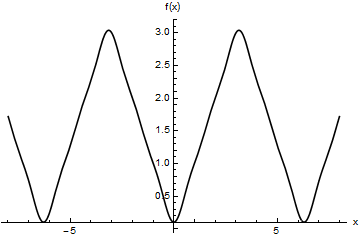
\includegraphics[scale=0.5]{fig/trigo-triangle-wave}
\caption{$\Lambda\Lambda\Lambda\Lambda\Lambda\Lambda$}
\label{fig-trigo-triangle-wave}
\end{figure}

这里有一项常数$\frac{\pi}{2}$,因为$f(x)$以$\frac{\pi}{2}$为中心,上下变化。如果没有常数,就只能以$0$为中心。

事实上,任何“好看”的周期函数都可以用一些(可能是无穷多个)三角函数加上一个常数“拼出来”。这个“好看”的意思要以后再讲,现在我们只要知道,连续函数或者在有限个点断掉的函数都可以(比如方波其实是在两条横线之间断掉),而$\frac{1}{x}$这样爆掉的函数就不行。至于“拼出来”是什么意思也要以后再讲。这样的级数就叫做傅立叶级数。

把任何函数表示成三角函数的和有一个好处。前面微分方程那里讲过,线性常系数非齐次微分方程(比如$x''+2 \beta x'+\omega_0^2 x=f(t)$)的右边表示系统受到的外力。外力为三角函数的情况我们已经会解了,而外力是其他函数的情况就没有这么容易解。

但是我们知道,如果$x''+2 \beta x'+\omega_0^2 x=f_1(t)$和$x''+2 \beta x'+\omega_0^2 x=f_2(t)$都可以解出来,那么$x''+2 \beta x'+\omega_0^2 x=f_1(t)+f_2(t)$的解可以直接通过线性叠加得到。因此可以把外力表示成三角函数的和,分别算出每个三角函数对应的解,然后线性叠加。

如果要研究电子元件中不同频率的交流电或者电磁波,也会用到傅立叶级数。打电话的时候会有嘶嘶的噪音,这些噪音的频率比说话声音的频率高,要除去噪音也可以用傅立叶级数。甚至地心说当中用多个圆轨道(本轮、均轮)来近似表示天体的椭圆轨道,也有这样的思想。
\section{算出傅立叶级数}
简单起见,只考虑周期为$2 \pi$的函数,其他周期函数可以在$x$前面乘系数来把周期变成$2 \pi$。已知一个函数$f(x)$的解析式,现在要把它表示为
\begin{equation*}
f(x)=\sum_{n=1}^{\infty} a_n \sin n x+\sum_{n=1}^{\infty} b_n \cos n x+c
\end{equation*}

要算出$f(x)$的傅立叶级数,关键是确定$a_n,b_n,c$这些系数。先来看这个积分:
\begin{equation*}
\int_{-\pi}^{\pi} \sin m x \sin n x \opd x
\end{equation*}

其中$m,n$都是整数。用复变函数那里讲过的方法可以算出,如果$m=n$,那么积分为$\pi$,否则为$0$。此外,
\begin{align*}
\int_{-\pi}^{\pi} \cos m x \cos n x \opd x&=\begin{cases} \pi, &m=n \\ 0, &m \neq n \end{cases} \\
\int_{-\pi}^{\pi} \sin m x \cos n x \opd x&=0 \\
\int_{-\pi}^{\pi} 1 \cdot \sin n x \opd x&=\int_{-\pi}^{\pi} 1 \cdot \cos n x \opd x=0
\end{align*}

所以我们可以干一件神奇的事情:计算$\int_{-\pi}^{\pi} \sin m x f(x) \opd x$,结果就是$\pi a_m$。$b_m$则可以乘$\cos m x$来确定。另外,$\int_{-\pi}^{\pi} f(x) \opd x=2 \pi c$。所以傅立叶级数是

\begin{equation*}
f(x)=\sum_{n=1}^{\infty} \left( \frac{1}{\pi} \int_{-\pi}^{\pi} \sin n x f(x) \opd x \right) \sin n x+\sum_{n=1}^{\infty} \left( \frac{1}{\pi} \int_{-\pi}^{\pi} \cos n x f(x) \opd x \right) \cos n x+\frac{1}{2 \pi} \int_{-\pi}^{\pi} f(x) \opd x
\end{equation*}

(这个公式又有积分又有求和可以拿来装逼)

至于怎么算出这些积分,不是我们现在关心的事情。即使知道$f(x)$的解析式,这些积分也不一定能用初等函数表示。实际情况下我们可能连$f(x)$的解析式都不知道,只能用实验来拟合,而这些积分也只要算出近似值。近似计算积分的方法我们以后再讲。

现在可以算出前面方波的傅立叶级数:
\begin{align*}
f(x)&=\begin{cases} -1, &-\pi<x<0 \\ 1, &0<x<\pi \end{cases} \\
a_n&=\frac{1}{\pi} \int_{-\pi}^{\pi} \sin n x f(x) \opd x \\
&=\frac{2}{\pi} \int_{0}^{\pi} \sin n x \opd x \\
&=\begin{cases} 0, &n \bmod 2=0 \\ \frac{4}{n \pi}, &n \bmod 2=1 \end{cases}
\end{align*}

根据奇偶性可以直接看出$b_n=\frac{1}{\pi} \int_{-\pi}^{\pi} \cos n x f(x) \opd x=0$,$c=\frac{1}{2 \pi} \int_{-\pi}^{\pi} f(x) \opd x=0$,这样就算出了前面的式子。

如果$f(x)$不是周期函数,这种方法会把它强行变成周期函数。比如$f(x)=x$,会变成
\begin{equation*}
f(x)=\begin{cases} f(x+2 \pi), &x \le -\pi \\ x, &-\pi<x \le \pi \\ f(x-2 \pi), &x>-\pi \end{cases}=2 \sum_{n=1}^{\infty} \frac{(-1)^{n+1}}{n} \sin n x=2(\sin x-\frac{1}{2} \sin 2 x+\frac{1}{3} \sin 3 x-\dots)
\end{equation*}

前$5$项如图\ref{fig-trigo-x}。(因此上面方波的解析式我没写$(-\pi,\pi)$以外的东西)
\begin{figure}[htb]
\centering
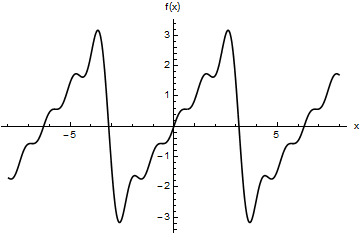
\includegraphics[scale=0.5]{fig/trigo-x}
\caption{就是把$(-\pi,\pi)$以内的东西往两边复制}
\label{fig-trigo-x}
\end{figure}
\section{函数的内积与正交}
你有没有觉得这件事情很神奇:$\int_{-\pi}^{\pi} \sin m x f(x) \opd x$可以把$f(x)$中除了$\sin m x$的项全部变成$0$,只剩下$\sin m x$对应的系数。现在我们来更深刻地理解这件事情。

如果两个函数$f(x),g(x)$的定义域都是$[a,b]$,可以定义它们的内积$\langle f(x),g(x) \rangle=\int_a^b f(x) g(x) \opd x$。内积是一种把两个函数变成一个实数的操作。

不仅是函数,其他东西也可以定义内积,比如两个实数的内积就是乘积,两个矢量$\mathbf{a},\mathbf{b}$的内积就是$\mathbf{a} \cdot \mathbf{b}$。

对于二维矢量,$\langle \mathbf{a},\mathbf{b} \rangle=a_x b_x+a_y b_y$。推广到$n$维矢量,$\langle \mathbf{a},\mathbf{b} \rangle=\sum_{i=1}^n a_i b_i$(用前面讲过的爱因斯坦求和约定,就是$\langle \mathbf{a},\mathbf{b} \rangle=a_i b_i$)。可以看出,函数内积就是把矢量内积的求和改成积分。

如果两个矢量的内积为$0$,说明这两个矢量垂直。如果两个函数的内积为$0$,我们说这两个函数“正交”,就是垂直的意思。$\sin m x$与$1$和$\cos n x$都正交,与$\sin n x(m \neq n)$也正交。

我们可以用三个相互正交的矢量$\mathbf{x},\mathbf{y},\mathbf{z}$(它们的模长不一定是$1$)作为坐标轴,建立三维直角坐标系,然后算出任何一个三维矢量$\mathbf{a}$在各个坐标轴上的分量,也就是把$\mathbf{a}$表示为$a_1 \mathbf{x}+a_2 \mathbf{y}+a_3 \mathbf{z}$。

现在可以这样理解傅立叶级数:用$\sin x,\sin 2 x,\sin 3 x,\dots,\cos x,\cos 2 x,\cos 3 x,\dots,1$这无穷多个相互正交的函数作为坐标轴,建立一个无穷多维的直角坐标系,然后算出任何一个函数$f(x)$在各个坐标轴上的分量,就是$a_n,b_n,c$这些系数。

也就是说,所有定义域为$[a,b]$的“好看”的函数构成一个线性空间,这个空间里的每个点对应一个函数。一个矢量在不同的坐标系里有不同的分量,但是矢量还是原来的矢量。同样,$a_n,b_n,c$这无穷多个系数表示的就是原来的函数。还可以把这个函数表示为泰勒级数$\sum_{n=0}^{\infty} a_n x^n$,这些系数$a_n$表示的仍然是原来的函数,只是换了一个“坐标系”而已。

怎么算出这些分量呢?矢量$\mathbf{a}$在$\mathbf{x}$上投影的长度是$\frac{\langle \mathbf{a},\mathbf{x} \rangle}{\sqrt{\langle \mathbf{x},\mathbf{x} \rangle}}$,与$|\mathbf{x}|$无关。但是把$\mathbf{x}$作为一根坐标轴的时候,$\mathbf{a}$在$\mathbf{x}$上的分量是$\frac{\langle \mathbf{a},\mathbf{x} \rangle}{\langle \mathbf{x},\mathbf{x} \rangle}$,$|\mathbf{x}|$越大,分量越小。这里$|\mathbf{x}|$不一定是$1$,它表示坐标轴上的单位长度。这样应该很容易理解$a_n=\frac{\langle f(x),\sin n x \rangle}{\langle \sin n x,\sin n x \rangle}$。

(说句题外话:记数法就是用线性空间来表示实数。比如十进制记数法中的个位、十位、百位……以及十分位、百分位……可以看成无数条坐标轴,每条坐标轴上的分量可以是$0,1,2,\dots,9$这些数字。十进制和二进制可以表示同一个数,只是换了一个“坐标系”。)
\section{复指数形式的傅立叶级数;傅立叶变换}
傅立叶级数中三角函数的频率都是整数(这里不区分频率和角频率,就是$\sin \omega x$中的$\omega$)。如果改成实数会怎么样呢?容易想到,前面的求和要改成积分,这就是傅立叶变换。(有些地方会把傅立叶级数也叫傅立叶变换,因为它实在太有名了)

先把傅立叶级数中的三角函数用复指数来表示,也就是$f(x)=\sum_{n=-\infty}^{\infty} a_n \rme^{\rmi n x}$,这样正弦、余弦和常数项就不用分开讨论了。现在$f(x)$和$a_n$可以是复数,但是自变量$x$还是实数,$x$是复数的情况以后再讲。

内积的定义也要作一些补充:$\langle f(x),g(x) \rangle=\int_{-\pi}^{\pi} f(x) g^*(x) \opd x$,${}^*$表示共轭复数。这样内积就不满足交换律了,$\langle f(x),g(x) \rangle=\langle g(x),f(x) \rangle^*$。如果$f(x)$和$g(x)$都是实数,内积还是和原来一样。

这样才能保证$\langle \rme^{\rmi m x},\rme^{\rmi n x} \rangle=\begin{cases} 2 \pi, &m=n \\ 0, &m \neq n \end{cases}$,$a_n=\frac{ \langle f(x),\rme^{\rmi n x} \rangle}{\langle \rme^{\rmi n x},\rme^{\rmi n x} \rangle}$。

(顺便说一下,即使$f(x)$是负数或者复数,$\langle f(x),f(x) \rangle$总是非负实数,跟绝对值或者模长的性质一样,我们可以定义函数$f(x)$的模长是$\sqrt{\langle f(x),f(x) \rangle}$)

如果$f(x)$的最小正周期是$T$,傅立叶级数要改成(求和后面的$\Delta n$原来是省略的)
\begin{align*}
f(x)&=\sum_{n=-\infty}^{\infty} a_n \rme^{\rmi n \frac{2 \pi}{T} x} \Delta n \\
a_n&=\frac{\langle f(x),\rme^{\rmi n \frac{2 \pi}{T} x} \rangle}{\langle \rme^{\rmi n \frac{2 \pi}{T} x},\rme^{\rmi n \frac{2 \pi}{T} x} \rangle} \\
&=\frac{\int_{-\frac{T}{2}}^{\frac{T}{2}} f(x) \rme^{-\rmi n \frac{2 \pi}{T} x} \opd x}{\int_{-\frac{T}{2}}^{\frac{T}{2}} \rme^{\rmi n \frac{2 \pi}{T} x} \rme^{-\rmi n \frac{2 \pi}{T} x} \opd x} \\
&=\frac{1}{T} \int_{-\frac{T}{2}}^{\frac{T}{2}} f(x) \rme^{-\rmi n \frac{2 \pi}{T} x} \opd x
\end{align*}

令$k=n \frac{2 \pi}{T}$,$\Delta n=\frac{T}{2 \pi} \Delta k$。这样$\Delta n$中有$T$,$a_n$中有$\frac{1}{T}$,两者可以消掉。令$g(k)=T a_n$,傅立叶级数变成$f(x)=\sum_{k=-\infty}^{\infty} g(k) \rme^{\rmi k x} \Delta k$。

现在终于可以把求和改成积分:$f(x)=\int_{-\infty}^{\infty} g(k) \rme^{\rmi k x} \opd k$,$g(k)=\frac{1}{2 \pi} \int_{-\infty}^{\infty} f(x) \rme^{-\rmi k x} \opd x$。

傅立叶变换中的$f(x)$是非周期函数,也就是$T \rightarrow \infty$,而固定$\Delta n=1$,所以$\Delta k \rightarrow 0$。$g(k)$称为$f(x)$的频谱。它是$k$的函数,与$x$无关。一些播放音乐的软件显示出的频谱(比如跳来跳去的柱子)就是它。

(一般$k$是波数,$x$是位置。这里就当$k$是频率,$x$是时间好了)

举个栗子:$f(x)=\rme^{-\frac{1}{2} x^2} \sin 10 x$,经过一些困难的计算可以得到$g(k)=-\frac{\rmi}{2} \rme^{-\frac{1}{2} k^2-50}(\rme^{10 k}-\rme^{-10 k})$,如图\ref{fig-gauss-sin10x}。
\begin{figure}[htb]
\centering
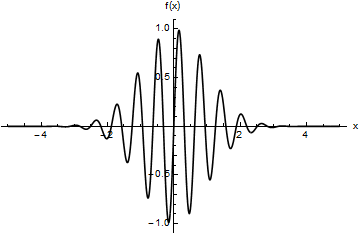
\includegraphics[scale=0.5]{fig/gauss-sin10x}
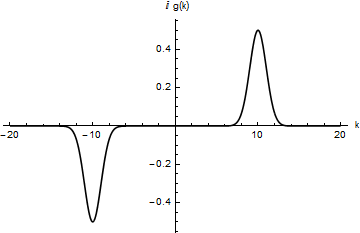
\includegraphics[scale=0.5]{fig/gauss-sin10x-g}
\caption{一下子举不出更简单的栗子,计算过程就不在这里讲了}
\label{fig-gauss-sin10x}
\end{figure}

我们来理解一下这个图像。首先,$\langle f(x),\rme^{\rmi k x} \rangle=\int_{-\infty}^{\infty} f(x) \rme^{-\rmi k x} \opd x$,积分的上下限是无穷大,只有$x \rightarrow \pm \infty$时$f(x) \rightarrow 0$,并且速度比$x^{-1}$更快,这个积分才存在,这样的函数才能进行傅立叶变换。所以$\sin 10 x$这样的周期函数反而不能进行傅立叶变换。

但是在现实生活中不可能有永远持续的振动,所有的振动都有开始和结束的时间。给$\sin 10 x$乘上一个“窗函数”$\rme^{-\frac{1}{2} x^2}$,它就能在无穷远处趋于$0$,而$0$附近的函数值不受太大影响。

许多正弦波叠加可以形成这样的图像,这些正弦波的频率主要在$10$附近。频率离$10$越远,对应的正弦波振幅越小。因为$f(x)$是奇函数,所以$g(k)$也是奇函数,而且是纯虚数,画图时已经乘了$\rmi$。

常见的窗函数还有$\begin{cases} 1, &-\frac{1}{2}<x<\frac{1}{2} \\ 0, &x<-\frac{1}{2} \text{或} x>\frac{1}{2} \end{cases}$(方形窗)和$\frac{1}{1+x^2}$(柯西窗)等等。

再举个栗子:$f(x)=\begin{cases} \cos 10 x, &-\frac{1}{2}<x<\frac{1}{2} \\ 0, &x<-\frac{1}{2} \text{或} x>\frac{1}{2} \end{cases}$,$g(k)=\sqrt{\frac{2}{\pi}} \frac{k \cos 5 \sin \frac{1}{2} k-10 \sin 5 \cos \frac{1}{2} k}{k^2-100}$,如图\ref{fig-block-sin10x}。
\begin{figure}[htb]
\centering
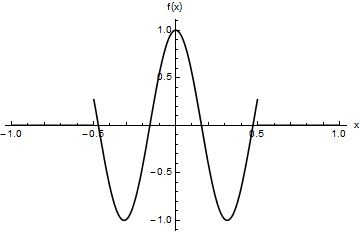
\includegraphics[scale=0.5]{fig/block-sin10x}
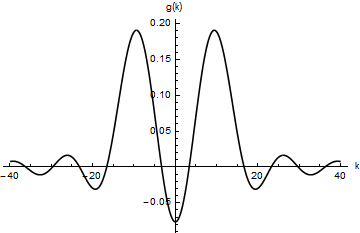
\includegraphics[scale=0.5]{fig/block-sin10x-g}
\caption{这次是偶函数}
\label{fig-block-sin10x}
\end{figure}

傅立叶变换可以用算符$\mathscr{F}$来表示:(这个花体的$\mathscr{F}$看起来很厉害,用下标来说明被变换和变换后的变量)
\begin{align*}
g(k)&=\mathscr{F}_{x \rightarrow k} f(x)=\frac{1}{2 \pi} \int_{-\infty}^{\infty} f(x) \rme^{-\rmi k x} \opd x &
f(x)&=\mathscr{F}^{-1}_{x \rightarrow k} g(k)=\int_{-\infty}^{\infty} g(k) \rme^{\rmi k x} \opd k
\end{align*}

为了对称性,有时候会调整系数$2 \pi$:(下面的公式一般用在量子力学之类的地方,上面的公式一般用在控制系统之类的地方,用的时候会注明)
\begin{align*}
g(k)&=\mathscr{F}_{x \rightarrow k} f(x)=\frac{1}{\sqrt{2 \pi}} \int_{-\infty}^{\infty} f(x) \rme^{-\rmi k x} \opd x &
f(x)&=\mathscr{F}^{-1}_{x \rightarrow k} g(k)=\frac{1}{\sqrt{2 \pi}} \int_{-\infty}^{\infty} g(k) \rme^{\rmi k x} \opd k
\end{align*}

量子力学和波动光学的最后几章是傅立叶变换的应用,你可以翻回去看看。
